\section{Description}\label{sec:description}
For this project I continued using the Evolutionary Algorithm(EA) that I
developed for the previous project. Because of the modularity in the previous
code not that much had to be changed apart from some minor changes to achieve
better performance. As with the last project when needing to adapt the EA to a
new problem one has to extend some core classes for which the default behaviour
is not appropriate. For this project all the extended code can be found in the
file \textit{neuron\.py} which contains all the code to simulate the task at
hand.

For this project I decided that I wanted to change the crossover function in the
genotype which meant that I had to extend the default genotype and create a new
class. This is quite easy and only the code for the crossover needed to be
changed. I will explain a bit more about why I wanted to change the default
crossover below, but for now in listing \ref{code:neuron-crossover} one can see
the code.

\lstinputlisting[language=Python, firstline=179, lastline=208,
	label=code:neuron-crossover, caption=The default genotype extended to
support a different kind of crossover more appropriate for the
problem.]{../src/neuron.py}

\subsection{Genotype}\label{sec:genotype-description}
Since the phenotype of the spiking neuron relied on some values being in a
certain range the code uses a variable amount of bits to represent these
variables. The number of bits is user configurable to allow for testing of
different sizes. The genotype then is just a bit array with 5xBITS where 5 represent
the five variables. Since the genotype is just an array of bits I decided that
for this project I would try out Gray Code to interpret those bits. This was
done to ensure that mutation would not have the large impact it would have if
regular conversion from a bit array to an integer was used. The genotype code
does not need to do anything extra in order for this to apply and only in the
conversion between genotype and phenotype is this extra bit of information used.

As mentioned above the crossover method was changed for this project. The change
enables the crossover to take into consideration each of the five variables.
This was done to make inheritance stronger. The change in code(listed in
\ref{code:neuron-crossover}) means that if we imagine the first variable
representing \textit{a} as the first 10 bits of the array, a child made from two
such parents would inherit 50\% of \textit{a} from one parent and another 50\%
from the other. There is no crossover between different variables which should
mean that the inheritance is stronger between parents and child and random bits
from a variable will not be put into another variable. To illustrate a bit
better I have tried to create an approximate figure in
\ref{fig:neuron-crossover}.

\begin{figure}[h]
	\centering
	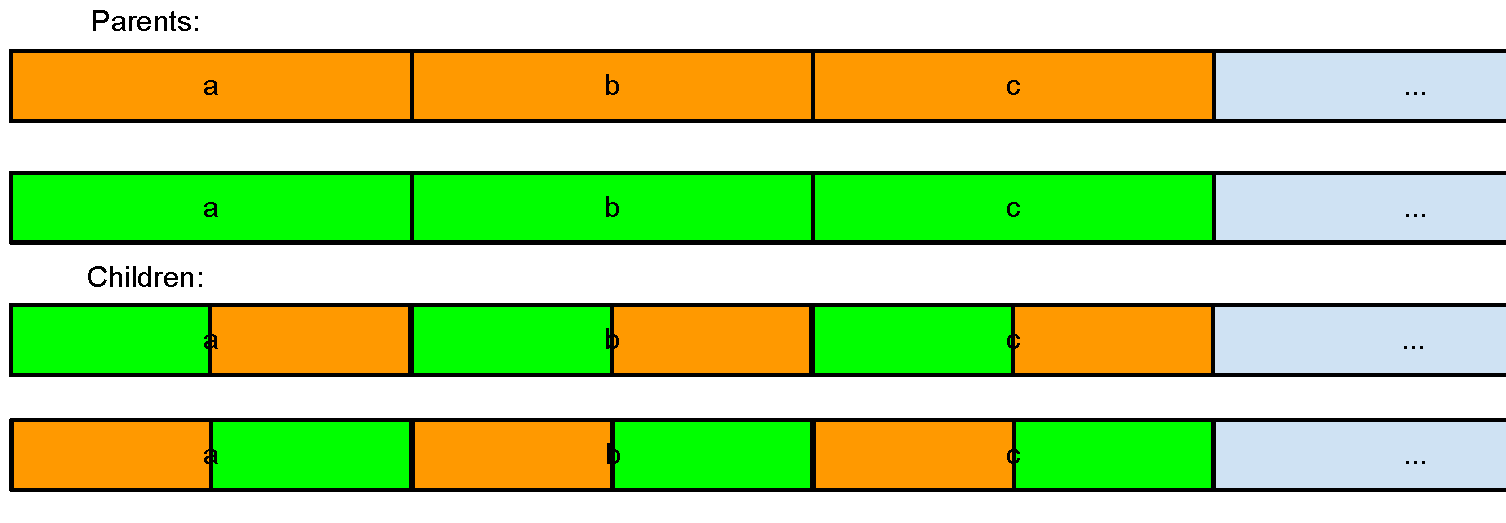
\includegraphics[scale=0.5]{crossover.pdf}
	\caption{A representation of crossover in the neuron}
	\label{fig:neuron-crossover}
\end{figure}

\subsection{Fitness}\label{sec:fitness-description}
To evaluate the fitness of each spike train I implemented the three different
distance metrics suggested in the assignment. Since those metrics evaluated
distance meaning a smaller distance is better and the EA code was set up for
larger is better the natural choice was to just do 1.0/f(x), where f(x) is one of
the three distance metrics. Since both \textit{Spike Time Distance Metric(STDM)}
and \textit{Spike Interval Distance Metric(SIDM)} needed the peaks I created one
more parent class which could calculate that. In listing \ref{code:SIDM} we can
see the minimal code needed for SIDM\footnote{Note that this code does not
include the code necessary for peak calculation}.

\lstinputlisting[language=Python, firstline=162, lastline=177, label=code:SIDM,
caption=The SIDM implementation]{../src/neuron.py}
